\section{Prüfung 09.02.2021}
\subsection{Echtzeit}
\subsubsection{a)}
Ein Fahrzeug benötigt 20 Sekunden zum Überqueren einer Kreuzung mit einer Ampel. Zeichnen Sie in
das folgende Diagramm den Profit/Penalty-Verlauf für die Operation „Fahrzeug fährt in Kreuzung ein“
für den Fall dass die Ampel zunächst 40 Sekunden Grün zeigt, dann 10 Sekunden Gelb und dann 40
Sekunden Rot.

\begin{figure}[H]
  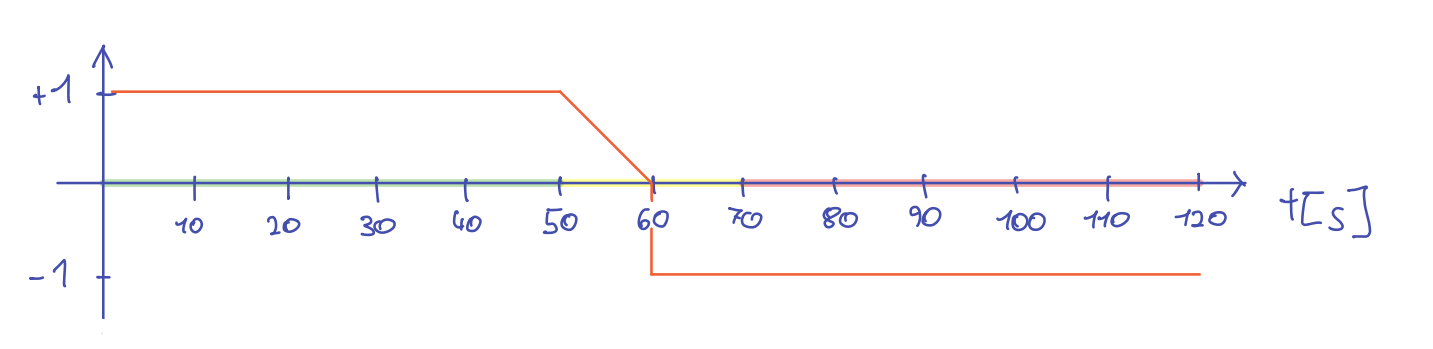
\includegraphics[width=10cm]{images/KA090221/1a.png}
  \centering
\end{figure}

\subsubsection{b)}
Handelt es sich hier um weiche, feste oder harte Echzeit? Begründen Sie!

Es handelt sich um harte Echtzeit, fährt das Auto zu spät in die Kreuzung ein kann es zu einem Schaden durch 
andere Autos kommen. Hier muss angenommen werden, dass wenn Rot aufleuchtet andere Autos schon wegfahren und 
nicht auf Autos in der Kreuzung achten.

\subsection{Busse}
\subsubsection{a)}
Warum ist Standard-Ethernet nicht echtzeitfähig?

Standard-Ethernet vewendet CSMA/CD und TCP/IP welche dieses Methode nicht echtzeitfähig macht. Es werden
Kollisionen detektiert. Gibt es eine Kollision wird eine zufällige Zeit gewartet und das Paket erneut angefordet.

\subsubsection{b)}
Was versteht man unter Arbitrierung und wie ist diese beim CAN-Bus realisiert?

Bus Arbitrierung bedeuted, dass immer nur eine Kommunikation zugleich stattfinden kann (alle nacheinander $\rightarrow$ bottleneck).
Arbitrierung entscheided wer senden darf.

All masters send identifiers at the same time. If a node hears a dominant bit
but sends it recessively, it withdraws, i.e. the message with the smallest
identifier has the highest priority (00...0) (see I2C bus).
CSMA/AMP: Carrier Sense Multiple Access with Arbitration on Message
Priority\footnote{Folien Kap2\_3 S47}

\subsubsection{c)}
Zwei I²C-Master sind mit einem gemeinsamen I²C-Bus verbunden und versuchen gleichzeitig Daten an
einen ebenfalls mit dem Bus verbundenen I²C-Slave zu senden. Die Adresse des Slave ist 0x7A (7-Bit
Adresse) und das Register in welches geschrieben wird ist 0x37. Nehmen Sie an, dass der erste Master
die Nutzdaten 0x6E und der zweite Master die Nutzdaten 0x63 in das Register schreibt. Welche
Symbol-Folge wird über die Daten-Leitung des I²C-Buses gesendet? Die folgenden Symbole werden
dabei verwendet: 

\begin{itemize}
  \item 0 für Bit 0
  \item 1 für Bit 1
  \item S für das Start-Signal
  \item P für das Stopp-Signal
  \item A für das ACK-Bit
\end{itemize}
Slave 0x7a = 111 1010\\
Register 0x37 = 0011 0111\\
Master1 0x6E = 0110 1110\\
Master2 0x63 = 0110 0011\\

Master2 sendet als erstes da Nutzdaten von Master2 $<$ Master1 sind. 
\begin{equation}
  S\underbrace{1111010}_{Slave addr}\underbrace{0}_{R/N}A\underbrace{00110111}_{Register addr}A\underbrace{01100011}_{payload}AP
\end{equation}

anschließend sendet Master1

\begin{equation}
  S\underbrace{1111010}_{Slave addr}\underbrace{0}_{R/N}A\underbrace{00110111}_{Register addr}A\underbrace{0110 0011}_{payload}AP
\end{equation}

\subsection{Echtzeit Scheduling}
Gehen Sie von folgenden drei periodischen Tasks aus:\\
Task1 = (1; 2),\\
Task2 = (1; 8),\\
Task3 = (k; 16)\\
Ein Task ist als Taskj = (Cj; Tj) definiert, wobei Cj die Ausführungszeit (Worst-Case) von Task j und Tj die
Periode von Task j ist. Wir benutzen das Task-Modell aus der Vorlesung, d.h. für jeden Task ist die Periode
identisch mit der Deadline, die Ausführungszeiten der Tasks sind konstant und so weiter. Alle Tasks sind
gleichzeitig zum Zeitpunkt 0 ausführungsbereit.
Analysieren Sie (ohne Zeichnen), die Schedulebarkeit mit EDF in Abhängigkeit von k. Bitte geben Sie alle
Werte von k in der Tabelle an für die ein EDF Schedule auf keinen Fall / eventuell / auf jeden Fall existiert.
Begründen Sie Ihre Antwort!

Nicht schedulbar für $k>6$.\\
Schedulbar für $k \leq 6$.

\subsection{Taskprioritäten}
\subsubsection{a)}
Definieren Sie den Begriff „unbeschränkte Prioritätsinvertierung“

An einer Prioritätsinversion sind mehrere Prozesse oder Threads mit unterschiedlicher Priorität und eine Ressource beteiligt. Besetzt ein
Task mit niedriger Priorität die Resource kann ein Task mit hoher Priorität nicht darauf zugreifen. 
\subsubsection{b)}
Kann es in einem System mit zwei Tasks zu einer unbeschränkten Prioritätsinvertierung kommen?
Begründen Sie!

Nein, für unbeschränkte Prioritätsinvertierung benötigt es mindestens 3 Tasks. Task3 wartet auf Task1, der von Task2 verdrängt wird.
\begin{figure}[H]
  \includegraphics[width=10cm]{images/KA090221/2_erklärung.png}
  \centering
\end{figure}
\url{https://de.wikipedia.org/wiki/Priorit%C3%A4tsinversion}

\subsubsection{c)}
Kann es durch Prioritätsinvertierung zum Verlust der Echtzeitfähigkeit kommen? Begründen Sie Ihre
Antwort!

Ja, dadurch dass die höhere Priorität Aufgabe blockiert wird kann es zur Unterbrechung von Zeitkritischen Aufgaben führen und somit
die Echtzeitfähigkeit beeinträchtigen.

\subsubsection{d)}
Erläutern Sie ein Verfahren um die unbeschränkte Prioritätsinvertierung zu vermeiden!

Ressource bekommt ebenfalls eine Priorität, die höher als die der höchstprioren sie nutzenden Task ist.
Nutzt eine Task die Ressource, nimmt sie temporär diese höhere Priorität an. Oder Priority Aging oder Priority Inheritance

\subsection{Statecharts}
Der folgende Programmcode wurde aus einem Statechart generiert. Zeichnen Sie den ursprünglichen
Statechart, tragen Sie auch die Namen aller Zustände sowie aller Ereignisse ein und markieren Sie alle
initialen Zustände so wie in Statecharts üblich!

\begin{lstlisting}
void P_fsm () {
  int state = R;
  while (1) {
    int a = update_a();
    int c = update_c();
    if (a) return;
    switch (state) {
      case R: if (c) { state = S; } break;
      case S: if (c) { state = R; } break;
    }
  } 
}

void Q_fsm () {
  int state = T;
  while (1) {
    int a = update_a();
    int b = update_b();
    if (b) return;
    switch (state) {
      case T: if (a) { state = T; } break;
    }
  }
}

void main () {
 int state = P;
 while (1) {
  switch (state) {
    case P: P_fsm(); state = Q; break;
    case Q: Q_fsm(); state = P; break;
  }
 }
}
\end{lstlisting}

\begin{figure}[H]
  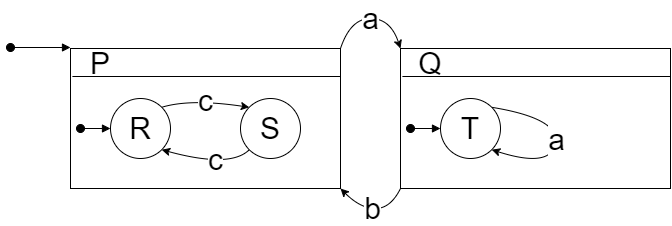
\includegraphics[width=10cm]{images/KA090221/3a.png}
  \centering
\end{figure}

\subsection{Speicherprogrammierbare Steuerung (SPS)}
Geben Sie zu folgendem Strukturierten Text eine Anweisungsliste und einen Funktionsplan an welche die
gleiche Funktion ausführen wie der folgende Strukturierte Text:
\begin{lstlisting}
  IF NOT A OR B THEN
    D := TRUE;
  ELSE
    D := FALSE;
  END_IF;
  Timer (IN:=D, PT:=#5s);
  C := Timer.Q;
\end{lstlisting}

\subsubsection{Anweisungsliste}
\begin{lstlisting}
  LD B
  ORN A
  ST D

  CAL Timer(IN:=D, PT:=#5s)
  LD Timer.Q
  ST C
\end{lstlisting}

\subsubsection{Funktionsplan}
\begin{figure}[H]
  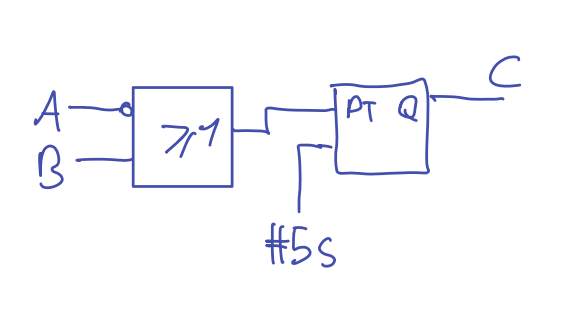
\includegraphics[width=10cm]{images/KA090221/6a.png}
  \centering
\end{figure}